\section{Passive Elemente}

\subsection{Widerstände}

\subsubsection{Definition}
\begin{multicols}{2}
\includegraphics[width=0.4\textwidth]{pictures/widerstand.png}

\columnbreak

$R=\rho\frac{l}{w*d}$
$\rho$: Spezifischer Widerstand
\end{multicols}


\subsubsection{Temperaturabhängige Widerstände}
\textbf{Thermistoren} sind Widerstände mit einer gezielt ausgeprägten
Temperaturabhängigkeit.\\Man unterscheidet:
\begin{itemize}
  \item PTC-Widerstände (Kaltleiter, positiver Temperaturkoeffizient): der
  Widerstandswert steigt mit steigender Temperatur
  \begin{itemize}
    \item verwendet als Temperatursensor
    \item als selbstrückstellende Sicherung
    \item als selbstregelndes Heizelement
    \item und zur Steuerung der Entmagnetisierung von Bildröhren
  \end{itemize}
  \item NTC-Widerstände (Heissleiter, negativer Temperaturkoeffizient): der
  Widerstandswert sinkt mit steigender Temperatur
  \begin{itemize}
    \item verwendet unter anderem als Temperatursensor
    \item und zur Einschaltstrombegrenzung
  \end{itemize}
\end{itemize}

\textbf{PTC}\\
\begin{figure}[htbs]
\includegraphics[scale=0.5]{pictures/ptc}
\end{figure}

\textbf{NTC}\\
\begin{minipage}{9cm}
\begin{equation}
R_{T}=R_{R}*e^{B*(\frac{1}{T}-\frac{1}{T_{R}})}
\end{equation}
\begin{tabular}{ll}
  $R_{T}$: &NTC resistance at temperature T in K\\
  $R_{R}$: &NTC resistance at rated temperature TR in K\\
  T: &Temperature in K\\
  $T_{R}$: &Rated temperature in K\\
  B: &B value, material-specific constant of NTC thermistor\\
  e: &Euler number (e = 2.71828)
\end{tabular}
\end{minipage}
\begin{minipage}{9cm}
\includegraphics[scale=0.5]{pictures/ntc}
\end{minipage}

\subsubsection{Fotowiderstände}
\begin{itemize}
  \item CdS-Fotowiderstand; die fotoempfindliche Widerstandsschicht befindet
  sich zwischen den kammartigen Kontaktflächen
  \item Ein Fotowiderstand ändert seinen Widerstand unter Lichteinwirkung.
  Trifft Licht auf die fotoempfindliche Fläche des Fotowiderstands, verringert
  sich der Widerstand durch den inneren fotoelektrischen Effekt.
\end{itemize}

\subsubsection{Spannungsabhängige Widerstände}
\begin{itemize}
  \item Sie werden Varistoren (ein aus „variabel“ und „Resistor“ gebildetes
  Kunstwort) genannt und bestehen aus Metalloxiden (meist dotiertes Zinkoxid).
  \item Sie verringern ihren Widerstandswert bei steigender Spannung, meist
  drastisch ab einer charakteristischen Schwellspannung ähnlich einer
  Zener-Diode (jedoch für beide Polariäten).
  \item Sie werden zur Begrenzung von Überspannungsimpulsen (Schwellspannungen
  von 5 Volt bis mehrere Kilovolt) eingesetzt, nicht jedoch zur Spannungsstabilisierung.
\end{itemize}

\subsubsection{Druck- und dehnungsabhängige Widerstände}
\begin{itemize}
  \item Dehnmessstreifen sind Folienwiderstände, die aufgeklebt werden. Sie
  ändern ihren Widerstandswert in Abhängigkeit ihrer Dehnung beziehungsweise
  Zugspannung.
\end{itemize}

\subsubsection{Verstellbare Widerstände, Potentiometer}
\begin{itemize}
  \item Potentiometer sind für häufiges Verstellen geeignet.
  \item ein beliebiger Widerstandswert zwischen zwei Grenzwerten einstellen
  \item Trimmpotentiometer (geringe Leistung) und Stellwiderstände (grosse
  Leistung) sind nur für gelegentliches Verstellen geeignet.
\end{itemize}


\subsection{Kondensatoren}
\begin{figure}[h]
\includegraphics[scale=0.4]{pictures/kondensatortypen}
\includegraphics[scale=0.4]{pictures/spannungkondensator}
\end{figure}

\subsubsection{Kapazitätswert}
\begin{minipage}{9cm}
\includegraphics[scale=0.8]{pictures/kapazitaetswert}
\end{minipage}
\begin{minipage}{9cm}
\begin{equation}
C=\varepsilon_{r}*\varepsilon_{0}*\frac{W*L}{d}=\varepsilon_{r}*\varepsilon_{0}*\frac{A}{d}
\end{equation}
mit $\varepsilon_{0}= 8.85 pF/m$
\end{minipage}

\subsubsection{Anwendungsgebiete}
\begin{longtable}{|l|l|}
\hline
\begin{minipage}{4cm}
\textbf{Keramik}
\end{minipage}
&
\begin{minipage}{6cm}
\begin{itemize}
  \item Konkurrenzlos bei hohen Frequenzen
  \item Werte bis 100uF
  \item Wichtigste Anwendung: Abblockkondensatoren bei IC-Speisung
\end{itemize}
\end{minipage}
\\
\hline
\begin{minipage}{4cm}
\textbf{Tantal, EL-Elko}
\end{minipage}
&
\begin{minipage}{6cm}
\begin{itemize}
  \item Polarisiert
  \item Einsatz v.a. bei Netzteilen
  \item Stützen von Speisung und Referenzspannungen
\end{itemize}
\end{minipage}
\\
\hline
\begin{minipage}{4cm}
\textbf{Film}
\end{minipage}
&
\begin{minipage}{6cm}
\begin{itemize}
  \item Filteranwendungen
\end{itemize}
\end{minipage}
\\
\hline
\end{longtable}
\subsubsection{Einschaltvorgang}
\input{idiotenseite/elektrotechnik/subsections/einschalt_kondensator}
\subsubsection{Ersatzschaltbild}
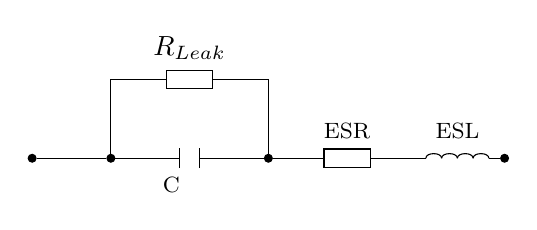
\begin{tikzpicture}

  \node (dot) at (1,1) [draw,circle,inner sep=1,fill]{};
  \node (dot2) at (2,1) [draw,circle,inner sep=1,fill]{};

  \node (c) at (3,1) [rectangle]{};
  \node (rleak) at (3,2)[draw,rectangle]{$~~~$};
  \node (dot3) at (4,1) [draw,circle,inner sep=1,fill]{};
  \node (esr) at (5,1)[draw,rectangle]{$~~~$};
  \coordinate (eslstart) at (6,1);
  \coordinate (eslend) at (6.8,1);
  \node (esl) at (6,1)[rectangle]{};
  \node (dot4) at (7,1) [draw,circle,inner sep=1,fill]{};

  \draw (dot) -- (dot2) -- (c) -- (dot3) -- (esr) -- (eslstart) (eslend) -- (dot4);
  \draw (dot2) |- (rleak) -| (dot3);

  \draw (c.south west) -- (c.north west);
  \draw (c.south east) -- (c.north east);

 \begin{scope}[out=90,in=90]
   \foreach \x in {0,0.2,0.4,0.6}
      \draw (eslstart)++(\x,0) to ++(0.2,0);
 \end{scope}

 \draw (rleak.north) node[above]{$R_{Leak}$};
 \draw (esr.north) node[above]{\footnotesize ESR};
 \draw (esl.north) node[above right]{\footnotesize ESL};
 \draw (c.south) node[below left]{\footnotesize C};


\end{tikzpicture}


\subsection{Induktivitäten/Spulen}
\begin{minipage}{9cm}
\begin{itemize}
  \item Eine Änderung des elektrischen Stromes erzeugt ein Magnetfeld, das der
  Stromänderung entgegenwirkt
  \item Masseinheit: Henry=AS/Vm
  \begin{gather}
  u_{i}=-N*\frac{d\Phi}{dt}\\
  L=\frac{N*\Phi}{I}
  \end{gather}
\end{itemize}
\end{minipage}
\begin{minipage}{9cm}
\includegraphics[scale=0.4]{pictures/induktivitaet}
\end{minipage}
\\
\begin{minipage}{9cm}
Ringspule\\
\begin{equation}
L=N^2*\frac{\mu_{0}\mu_{r}A}{2\pi r}
\end{equation}
\end{minipage}
\begin{minipage}{9cm}
\includegraphics[scale=0.4]{pictures/ringspule}
\end{minipage}
\\
\begin{minipage}{9cm}
Zylinderspule\\
\begin{equation}
L=N^2*\frac{\mu_{0}\mu_{r}A}{l}
\end{equation}
\end{minipage}
\begin{minipage}{9cm}
\includegraphics[scale=0.4]{pictures/zylinderspule}
\end{minipage}

\subsubsection{Einsatzgebiete und Schwerpunkte}
\begin{longtable}{|p{3.5cm}|l|l|l|l|l|}
\hline
\textbf{Application}&Inductance&Current rating&Resonance frequency&Q factor&DC
resistance\\
\hline
\textbf{RF circuits, resonant circuits}&low&low&very high&very high&low\\
\hline
\textbf{EMC}&high&high&high&low&very low\\
\hline
\textbf{RFID}&*&low&high&high&low\\
\hline
\textbf{DC/DC converters}&*&high&medium&high&low\\
\hline
\textbf{Transformers in DC/DC}&*&*&medium&*&low\\
\hline
\textbf{Signal processing}&*&low&high&-&medium\\
\hline
\end{longtable}

\subsubsection{Zusammenfassung}
\begin{itemize}
  \item Spulen sind relativ teuer
  \begin{itemize}
    \item In aktiven Filtern of durch aktive RC-Schaltungen ersetzt
  \end{itemize}
  \item Haupt-Einfastzgebiete
  \begin{itemize}
    \item DC-DC-Wandler
    \item Transformer: Galvanische Trennung
    \item Hochfrequenzanwendungen
    \item Entstörung (EMV, Datenübertragung)
  \end{itemize}
\end{itemize}

\subsubsection{Einschaltvorgang}
\input{idiotenseite/elektrotechnik/subsections/einschalt_spule}

\subsubsection{Ersatzschaltbild}
\begin{tikzpicture}

  \node (dot) at (1,1) [draw,circle,inner sep=1,fill]{};
  \node (dot2) at (2,1) [draw,circle,inner sep=1,fill]{};

  \node (c) at (3.5,2) [rectangle]{};
  \node (l) at (3,1)[rectangle]{};
  \coordinate (lstart) at (2.6,1);
  \coordinate (lend) at (3.4,1);
  \node (rcu) at (4,1)[draw,rectangle]{$~~~$};
  \node (dot3) at (5,1) [draw,circle,inner sep=1,fill]{};
  \node (dot4) at (6,1) [draw,circle,inner sep=1,fill]{};

  \draw (dot) -- (dot2) -- (lstart) (lend) --(rcu)  -- (dot3)  -- (dot4);
  \draw (dot2) |- (c) -| (dot3);

  \draw (c.south west) -- (c.north west);
  \draw (c.south east) -- (c.north east);

 \begin{scope}[out=90,in=90]
   \foreach \x in {0,0.2,0.4,0.6}
      \draw (lstart)++(\x,0) to ++(0.2,0);
 \end{scope}

 \draw (rcu.south) node[below]{\footnotesize $R_{Cu}$};
 \draw (l.south) node[below]{\footnotesize L};
 \draw (c.north) node[above]{\footnotesize $C_p$};

\end{tikzpicture}


